%----------------------------------------------------------------------------------------
%	PACKAGES AND OTHER DOCUMENT CONFIGURATIONS
%----------------------------------------------------------------------------------------

\documentclass[landscape,a0paper,fontscale=0.285]{baposter} % Adjust the font scale/size here

\usepackage{graphicx} % Required for including images
\graphicspath{{figures/}} % Directory in which figures are stored

\usepackage{amsmath} % For typesetting math
\usepackage{amssymb} % Adds new symbols to be used in math mode

\usepackage{booktabs} % Top and bottom rules for tables
\usepackage{enumitem} % Used to reduce itemize/enumerate spacing
\usepackage{palatino} % Use the Palatino font
\usepackage{wrapfig}
\usepackage[font=small,labelfont=bf]{caption} % Required for specifying captions to tables and figures

\usepackage{multicol} % Required for multiple columns
\setlength{\columnsep}{1.5em} % Slightly increase the space between columns
\setlength{\columnseprule}{0mm} % No horizontal rule between columns

\usepackage{tikz} % Required for flow chart
\usetikzlibrary{shapes,arrows} % Tikz libraries required for the flow chart in the template

\newcommand{\compresslist}{ % Define a command to reduce spacing within itemize/enumerate environments, this is used right after \begin{itemize} or \begin{enumerate}
\setlength{\itemsep}{1pt}
\setlength{\parskip}{0pt}
\setlength{\parsep}{0pt}
}

\definecolor{lightblue}{rgb}{0.5976,0,0} % Defines the color used for content box headers

\begin{document}

\begin{poster}
{
headerborder=closed, % Adds a border around the header of content boxes
colspacing=1em, % Column spacing
bgColorOne=white, % Background color for the gradient on the left side of the poster
bgColorTwo=white, % Background color for the gradient on the right side of the poster
borderColor=lightblue, % Border color
headerColorOne=black, % Background color for the header in the content boxes (left side)
headerColorTwo=lightblue, % Background color for the header in the content boxes (right side)
headerFontColor=white, % Text color for the header text in the content boxes
boxColorOne=white, % Background color of the content boxes
textborder=roundedleft, % Format of the border around content boxes, can be: none, bars, coils, triangles, rectangle, rounded, roundedsmall, roundedright or faded
eyecatcher=true, % Set to false for ignoring the left logo in the title and move the title left
headerheight=0.1\textheight, % Height of the header
headershape=roundedright, % Specify the rounded corner in the content box headers, can be: rectangle, small-rounded, roundedright, roundedleft or rounded
headerfont=\Large\bf\textsc, % Large, bold and sans serif font in the headers of content boxes
%textfont={\setlength{\parindent}{1.5em}}, % Uncomment for paragraph indentation
linewidth=2pt % Width of the border lines around content boxes
}
%----------------------------------------------------------------------------------------
%	TITLE SECTION 
%----------------------------------------------------------------------------------------
%
{
\includegraphics[height=4em]{logo.jpg}} % First university/lab logo on the left
{\bf\textsc{ETERNITY: NUMBERS - SILVER RATIO ($\delta s$)}} % Poster title
{\textsc{\{ Samir Anghan, Student id: 40040308, Team-A, SOEN 6481 \} 
\\ \{ Gina Cody School of Engineering and Computer Science, Concordia University \} }} % Author names and institution


%----------------------------------------------------------------------------------------
%	OBJECTIVES
%----------------------------------------------------------------------------------------

\headerbox{What was the objective? \& What activities were carried out?}{name=objectives,column=0,span=3,row=0}{

\textbf{Objective:} The purpose of the project was to carry out a number of activities (related to software systems requirements specification), resulting in a set of interrelated artifacts for the given problem domain.\\
\textbf{Problem Domain:}  A calculator that facilitates for certain calculations relating irrational numbers. \\
\textbf{Assigned Irrational Number:} Silver Ratio Number ($\delta s$) \\ \\
\textbf{Activities carried out: }


\begin{enumerate}\compresslist
\item Learning about the silver ratio number to attain sufficient background of the problem domain; Finding out unique characteristics of the silver ratio number.
\item Finding out a suitable interviewee; Preparing interview questions together in a project team; Conduct an interview of a potential user of ETERNITY: NUMBERS.
\item Collaboratively brainstorming and mind mapping with my team members to decide a persona template; Creating a persona based on my analysis of the interview.
\item Constructing a problem domain model for silver ratio number using UML; Constructing two different views of a use case model using UML. 
\item Eliciting, deciding, and creating a set of user stories. 
\item Creating a backward traceability matrix for user stories.
\item Implementing the user stories.  
\end{enumerate}

\vspace{0.3em} % When there are two boxes, some whitespace may need to be added if the one on the right has more content
}

%----------------------------------------------------------------------------------------
%	CRITICAL DECISIONS
%----------------------------------------------------------------------------------------

\headerbox{What critical decisions were made?}{name=decisions,column=0,row=1,below=objectives, above=bottom}{ % This block's bottom aligns with the bottom of the conclusion block

\begin{center}
    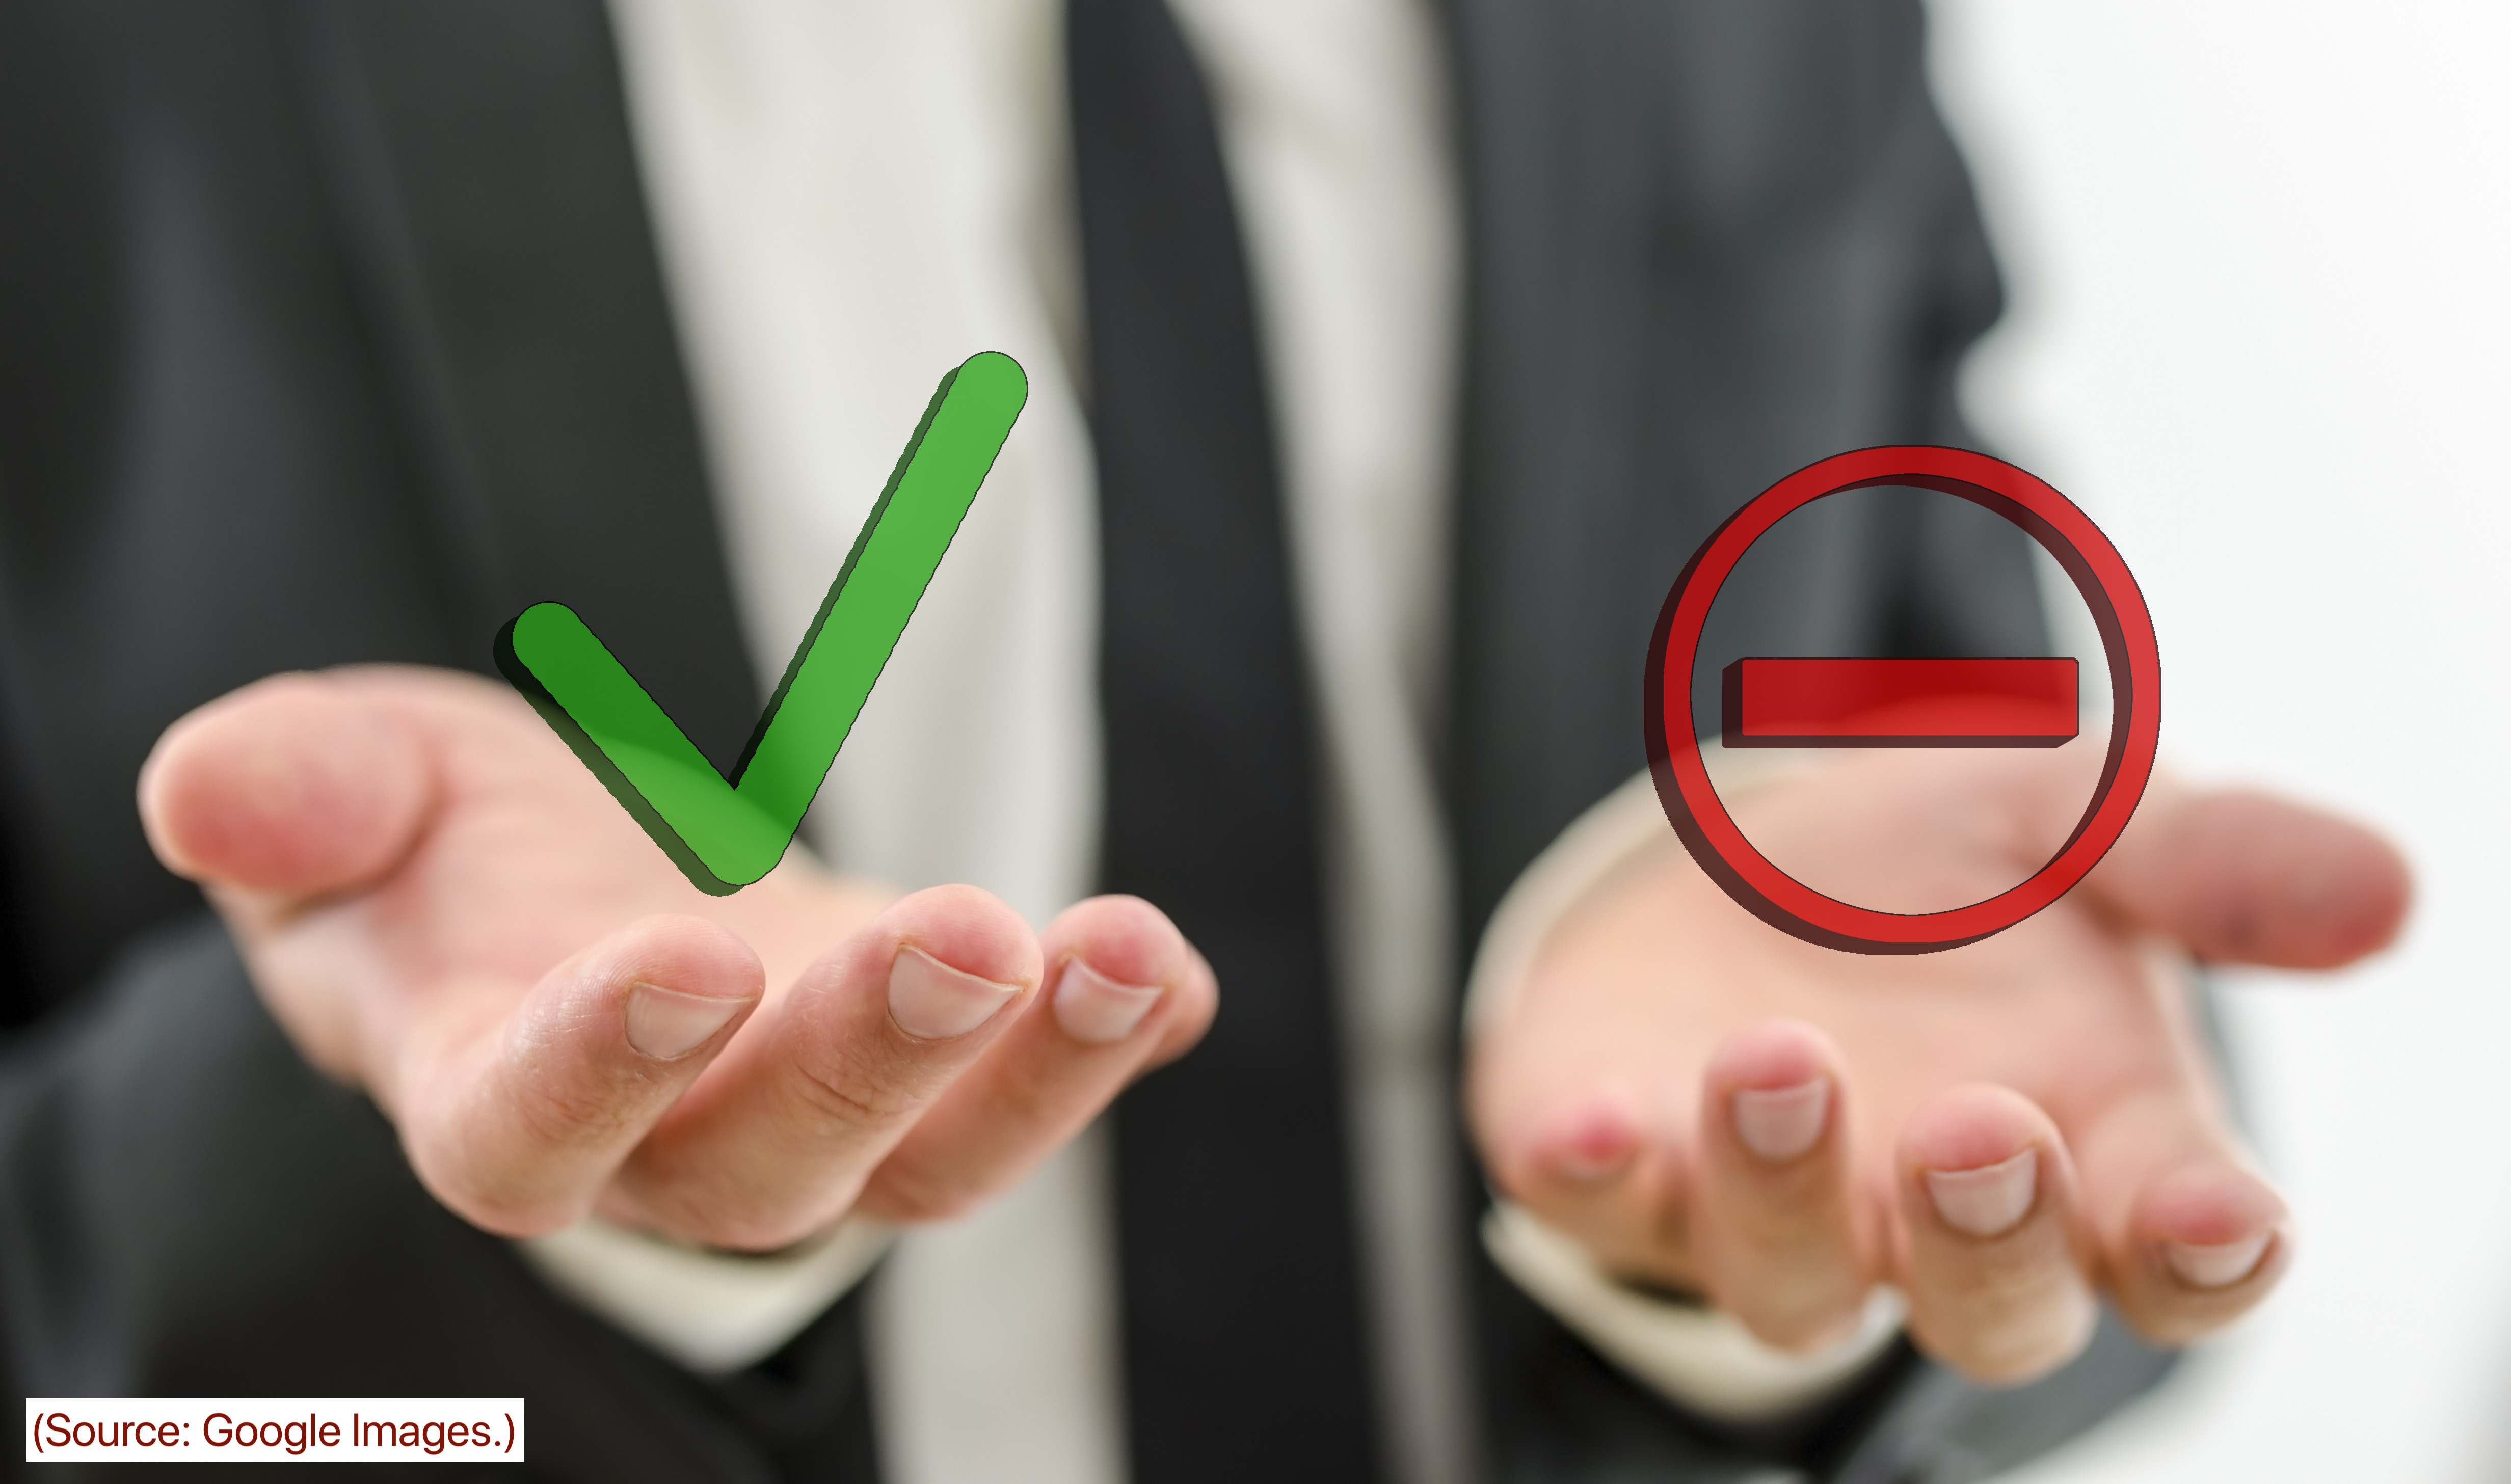
\includegraphics[height=4em]{decisions.jpeg}
\end{center}

\begin{description}\compresslist
\item[Situation:] \textbf{How many decimals of silver ratio number do I really need?}  \\
\item[Why it was critical?] Since a silver ratio is an irrational number and its value is 2.414213562373095048...$n$ ($where, 0\leq n\leq9$), one cannot write it in its exact form using only fractions or decimal numbers. The applications of the silver ratio number (such as an equation to find the area of a regular octagon) use the value of the silver ratio number in its equation. So, it becomes the matter of precision and accuracy. Hence, it is critical to the calculator system.\\

\item[Action:] Java's native and supported primitive datatype for precision is ``double'' which has a binary format that occupies 64 bits (8 bytes) and its significand has a precision of 53 bits (about 16 decimal digits).  Hence, I decided to consider maximum (supported by Java) that is 15 decimal digits (one decimal is reserved for the decimal number before decimal point). \\
\item[Result:] I considered 2.414213562373095 as a value of the silver ratio number by keeping in mind that calculating an area of an regular octagon \textbf{with full precision is not possible.}

\end{description}
}

%----------------------------------------------------------------------------------------
%	CHALLENGES & DIFFICULTIES
%----------------------------------------------------------------------------------------

\headerbox{What difficulties were faced?}{name=challenges,column=1,row=1,below=objectives}{ % This block's bottom aligns with the bottom of the conclusion block

\begin{center}
    
\includegraphics[height=4em]{problems.jpg}
\end{center}

Following are the difficulties I faced during project work:
\begin{itemize}\compresslist
\item Finding out a suitable interviewee who is using (or ever used) the silver ratio number.\\
\item Finding out the applications of the silver ratio number. \\

\end{itemize}
}

%----------------------------------------------------------------------------------------
%	LESSONS 
%----------------------------------------------------------------------------------------

\headerbox{What lessons are learned?}{name=lessons,column=2,row=1,below=objectives}{ % This block's bottom aligns with the bottom of the conclusion block

\begin{center}
    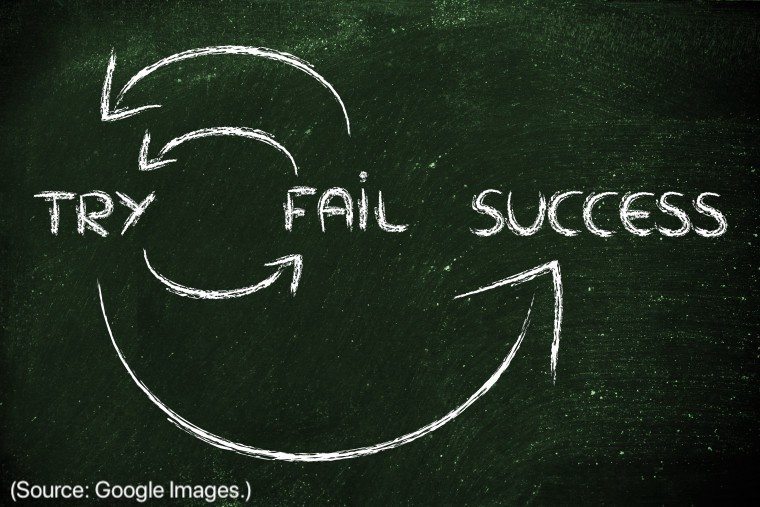
\includegraphics[height=4em]{lesson.jpeg}
\end{center}

\begin{itemize}\compresslist
\item Even though we were assigned with weakly-coupled teamwork, we had to work on persona and interview questions collaboratively. \textbf{I realized and learned that working in a team is not just working with others, it requires openness, being polite and communicative with other team members} because each team member had individual perspectives and different opinions.\\
\item Role-based requirements gathering is an important part of software requirements gathering and also it is crucial to the success of software development.\\
\item Persona should have clear, helpful and relevant description to the problem domain. \\
\end{itemize}

}

%----------------------------------------------------------------------------------------
%	WORKED WELL
%----------------------------------------------------------------------------------------

\headerbox{What worked well?}{name=workedwell,column=1,row=2,above=bottom,below=challenges}{

\begin{center}
    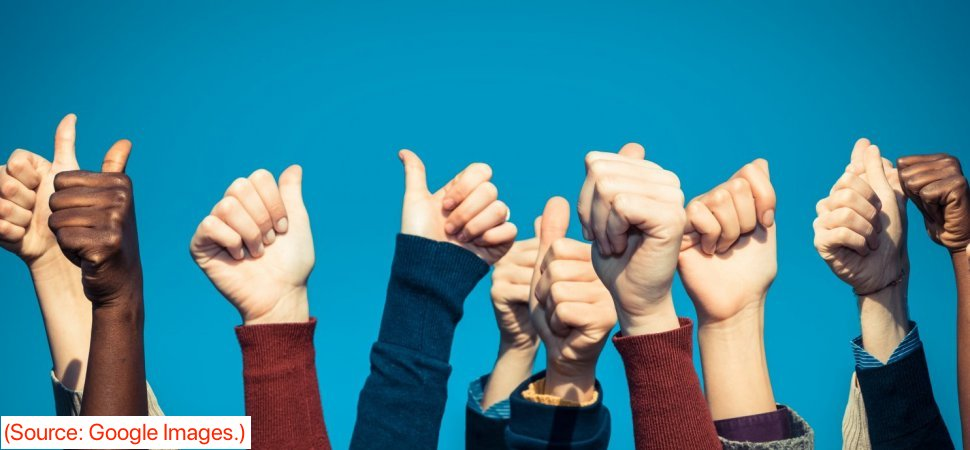
\includegraphics[height=4em]{workedwell.jpg}
\end{center}

\begin{itemize}\compresslist
\item Brainstorming and mind mapping with my team members to decide a persona
template and interview questions. \\
\item Conducting an interview of a potential user of the silver ratio number.\\
\item Learning LATEX report writing and documenting with  LATEX typeset.
\end{itemize}

}


%----------------------------------------------------------------------------------------
%	IMPROVEMENT
%----------------------------------------------------------------------------------------

\headerbox{What could be improved?}{name=improvements,column=2,row=2,above=bottom,below=lessons}{

\begin{center}
    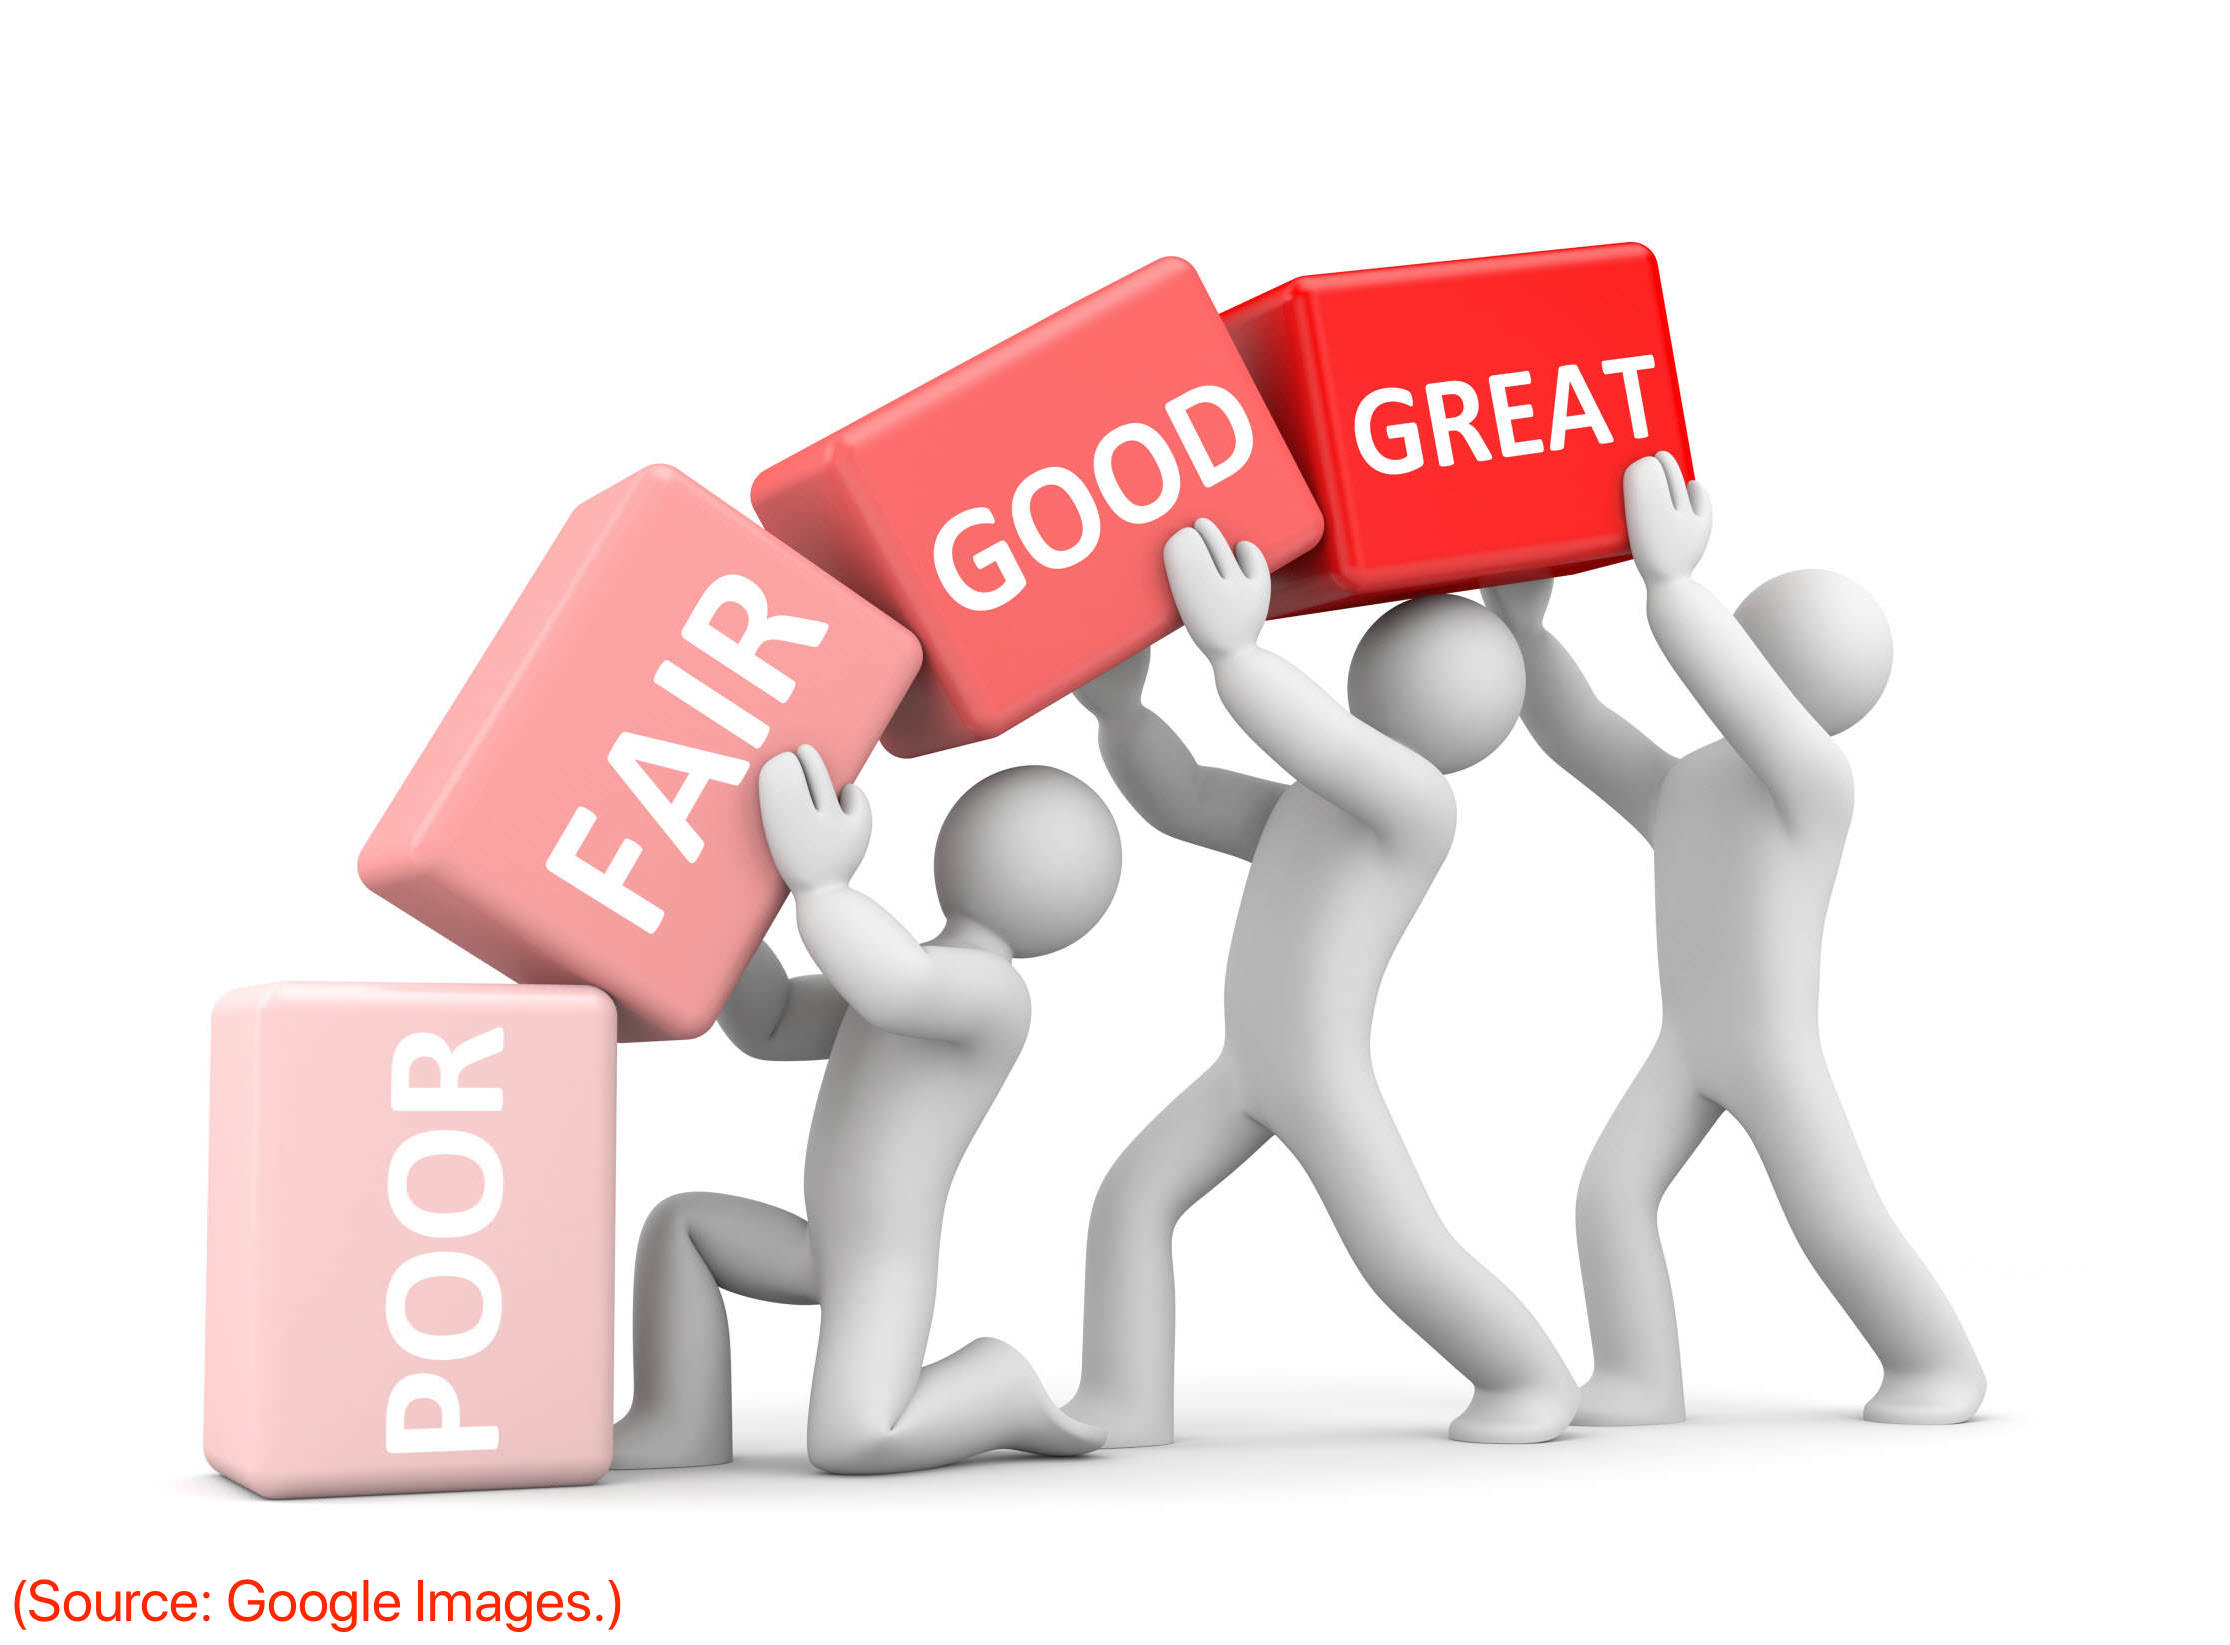
\includegraphics[height=4em]{improvement.jpg}
\end{center}
\begin{itemize}\compresslist
\item Implemented user stories could have been tested by writing unit tests. 
\end{itemize}
}

\end{poster}
\end{document}